\chapter{Isoviscous elastic-plated  gravity current model  for shallow
  magmatic intrusion}

\label{chap2} 
\minitoc

\section{Original theoretical framework}
\label{sec:orig-theor-fram}

Vertical  dyke propagation  through an  elastic medium  has been  well
studied    \citep{Lister:1991ut,Rubin:1995upa}.      In    particular,
\citet{Lister:1990hz} have shown  that, except in the  dyke head where
elastic forces play an important role, the dynamics of magma in feeder
dikes is  controlled by  a local balance  between buoyancy  forces and
viscous pressure drop.   At large depth in the crust,  the dynamics of
sills  and dikes  are  comparable  \citep{Lister:1991ut}.  At  shallow
depth,  however, geological  and  structural studies  have shown  that
magma makes room for itself mainly  by upward bending of the overlying
strata  \citep{Johnson:1973ho,Pollard:1973ho,E:2015tl}.   Most of  the
research on shallow horizontal magmatic intrusions have thus primarily
focused  on the  static  deformation of  the  overburden using  linear
elastic plate theory \citep{Johnson:1973ho,Koch:1981if}.

\begin{figure}
  \begin{center}
    \graphicspath{ {/Users/thorey/Documents/These/Manuscript/Figure/Chapter2/} }
    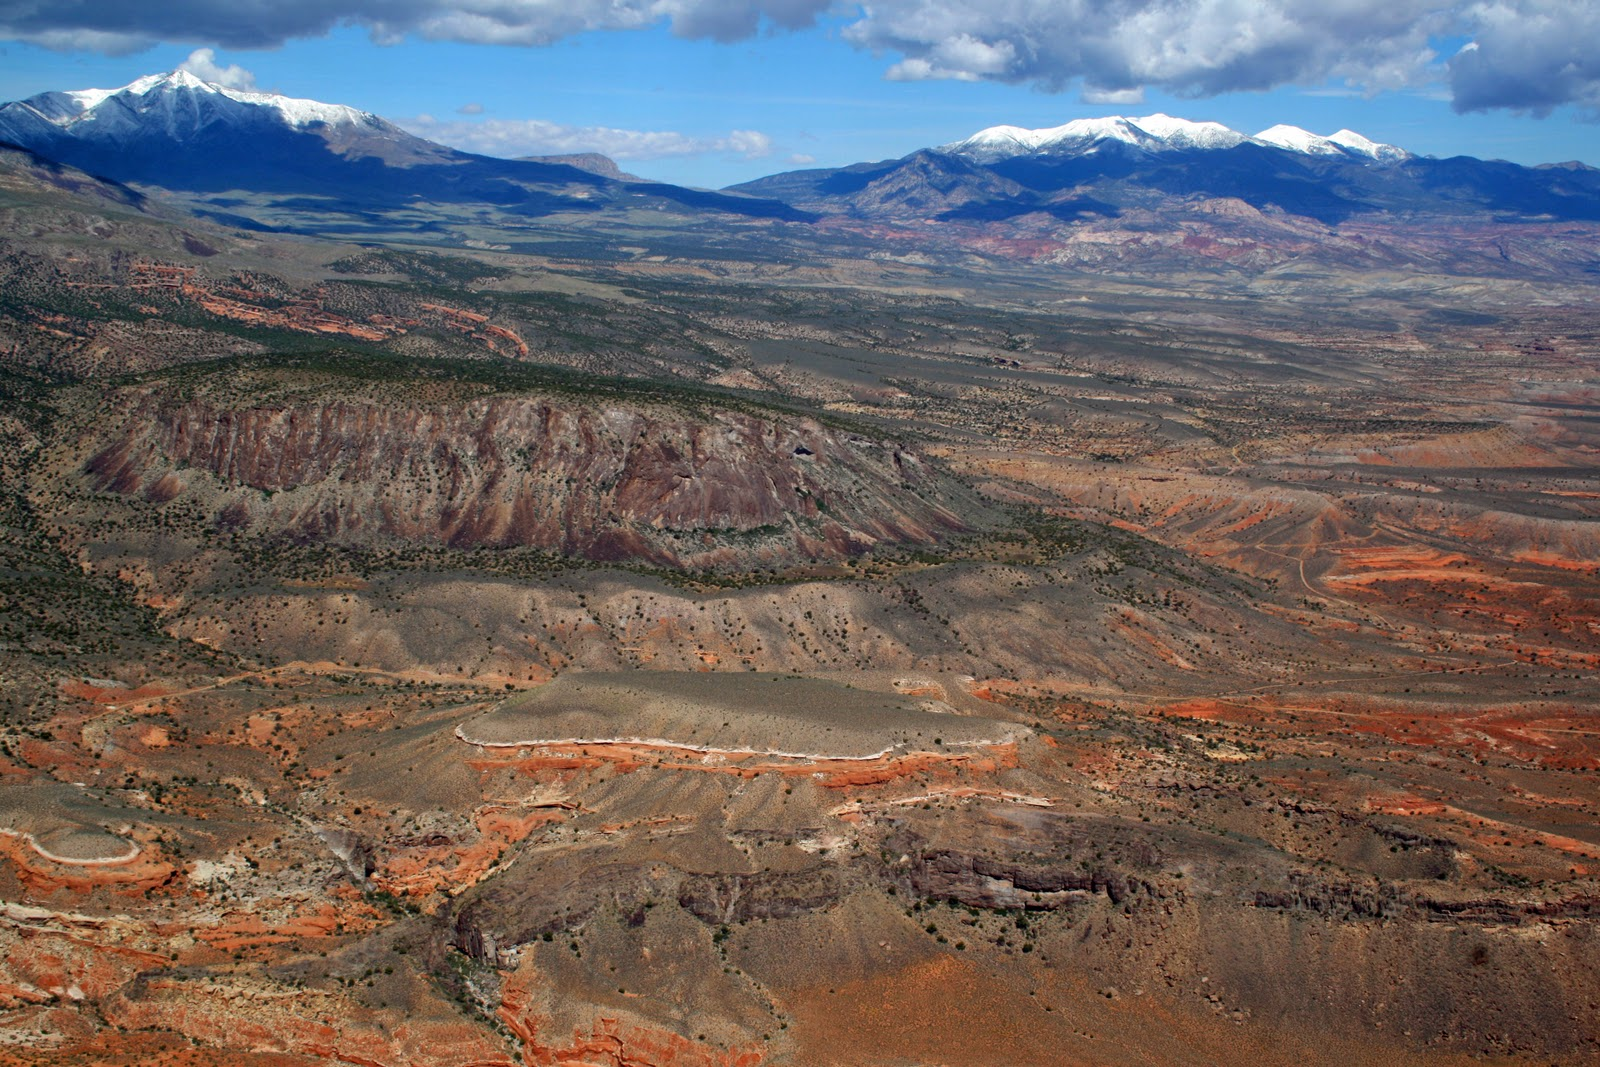
\includegraphics[scale=0.2]{IMG_2888a.jpg}
    \caption{ Dominating  the left center  of the  photo are a  few of
      Hillers'  well studied  satellite intrusions,  the cliff-forming
      outcrops of  the Black  Mesa bysmalith  (center), and  at bottom
      center, the Maiden Creek  sill. Photography courtesy, Jack Share
      \url{http://written-in-stone-seen-through-my-lens.blogspot.fr/2011/11/flight-plan-part-iii-henry-mountains.html}.}
    \label{Hillers}
  \end{center}
\end{figure}


In this static  framework, sill and laccolith have  been considered as
two    different    stages    of   the    same    intrusion    process
\citep{Johnson:1973ho,Pollard:1973ho,E:2015tl}:   a  first   stage  of
horizontal expansion  forming a sill  characterized by a  small aspect
ratio, and  a second stage  of vertical  thickening by bending  of the
overburden when the sill has became  sufficiently large to lift up the
overlying layer. At  the tip, the elastic  pressure eventually becomes
larger than the fracture toughness of the surrounding rocks

More recently, suggestion that laccoliths  can develop and grow by the
vertical  stacking  of  individual  and  successive  sills  have  been
supported by many  geological observations \citep{Menand:2008du}.  For
instance,  details studies  of  the small  satellite  intrusion of  Mt
Hiller,  in  the Henry  Mountain,  support  the formation  of  shallow
magmatic intrusions  by multiple  magma pulses  instead of  one single
feeding    episode    \citep{Morgan:2005km,Horsman:2009gea}    (Figure
\ref{Hillers}).   For instance,  the Trachyte  Mesa laccolith,  in the
Henry Mountains, have  been decomposed in a dozens  of separate sills.
This   suggestion  is   in  agreement   with  the   recent  model   of
\citep{Kavanagh:2006ig,Menand:2008du} where  sill where sills  form at
the interface  between soft  strata overlaid by  comparatively stiffer
strata as  discussed in the previous  chapter. Indeed, as a  sill form
and solidifies, it  generates a rigidity contrast with  the rock above
and  below  it.   Therefore,  sill emplacement  provide  a  favourable
emplacement of other sill, either  above if the rigidity of solifidied
sill is less ridig  than the surrounding or below if  it is more rigid
than the surrounding (Figure \ref{Horsmann}).

\begin{figure}
  \begin{center}
    \graphicspath{ {/Users/thorey/Documents/These/Manuscript/Figure/Chapter1/} }
    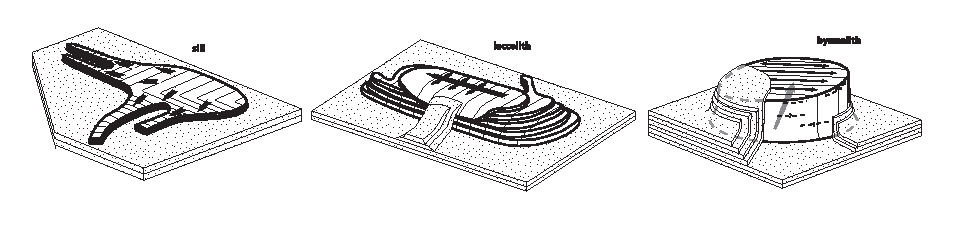
\includegraphics[scale=0.8]{Horsmann.eps}
    \caption{These  diagram, reproduced  from \citet{Horsman:2009gea},
      show characteristic features of  intrusions with sill, laccolith
      and bysmalith geometries assembled from multiple pulses.}
    \label{Horsmann}
  \end{center}
\end{figure}

Some   geological  studies   also   suggest  that   intermediate‐scale
intrusions form by  amalgamation of small magma sheets  [Habert and de
Saint‐Blanquat,  2004; Horsman  et al.,  2005]. However,  such studies
also show that  the emplacement of these intrusions must  occur over a
short enough  time scale for the  intrusion to keep a  melted core. In
the Black  Mesa intrusion  for instance,  solid state  textures around
internal contacts  between sheets are absent  and contact metamorphism
at the  periphery of the intrusion  is not significant; Habert  and de
Saint‐Blanquat [2004]  thus estimated  that this  body formed  in less
than  ∼100 years.   Hence,  if intermediate‐scale  intrusions form  by
amalgam-  ation of  small sheets,  with a  short repose  time interval
between intrusions, (i.e., such that a melted zone still exists), then
the whole intrusion behaves and deforms as a single flow.

However, magma viscosity and  injection rate necessarily influence the
dynamics of  sills and laccoliths.  The  own weight of the  magma also
induces a hydrostatic pressure  gradient through thickening which adds
to  the driving  pressure  and  must influence  the  spreading of  the
flow. In the  following, In this paper, I develop  a theoretical model
for  the spreading  of  shallow  depth intermediate‐scale  intrusions,
where magma, that is continuously injected at the intrusion center, is
accommodated by  roof lifting.  The  model differs from  the classical
static laccolith  model of  Turcotte and Schubert  [1982] in  that the
length of the flow is self  con- sistently determined.  The own weight
of  the magma  was neglected  in previous  models on  laccolith growth
[Kerr and  Pollard, 1998]; it  is taken into  account here as  it also
induces pressure gradients that drive the flow horizontally.

\section{Elastic-plated gravity current}
\label{C2-sec:model}

\citet{Michaut:2011kg} proposed  a new  model for  the spreading  of a
shallow   depth   intermediate-size   intrusions,   where   magma   is
continuously injected at the center and is accommodated by the bending
of  the  overlying strata.   In  particular,  the model  differs  from
previous ones  by considering  the driving  force associated  with the
magma weight which was neglected in older models.


In particular, the  model differ from the  previous attempts intrusion
by considering  the dynamics of the  spreading itself in a  sense that
the radius is self consistently determined.


Such  system  is  commonly  modeled as  an  isoviscous  elastic-plated
gravity current,  i.e.  an isoviscous  fluid spreading beneath  a thin
elastic   sheet  of   thickness  $d_c$   and  above   a  rigid   layer
\citep{Michaut:2011kg,Bunger:2011cb}  (Figure  \ref{C2-Sketch}).   The
behavior  of  isoviscous  elastic-plated  gravity  current  have  been
largely  discussed   in  the  past   few  years  in   both  carthesian
\citep{Michaut:2011kg,Bunger:2011cb,Anonymous:QWXp_4JV}            and
axisymmetrical  geometry  \citep{Michaut:2013dr,Lister:2013ia}.   This
section details  a summary of the  results for an isoviscous  fluid of
density $\rho_m$ and  viscosity $\eta$, supplied at  a continuous rate
$Q(t)$ through a cylindrical conduit of diameter $a$ at the center, in
an axisymmetrical  geometry (Figure \ref{C2-Sketch}). This  model will
constitute the reference for more elaborate models in the manuscript.

\begin{figure}[htbp]
  \begin{center}
    \graphicspath{ {/Users/thorey/Documents/These/Manuscript/Figure/Chapter2/} }
    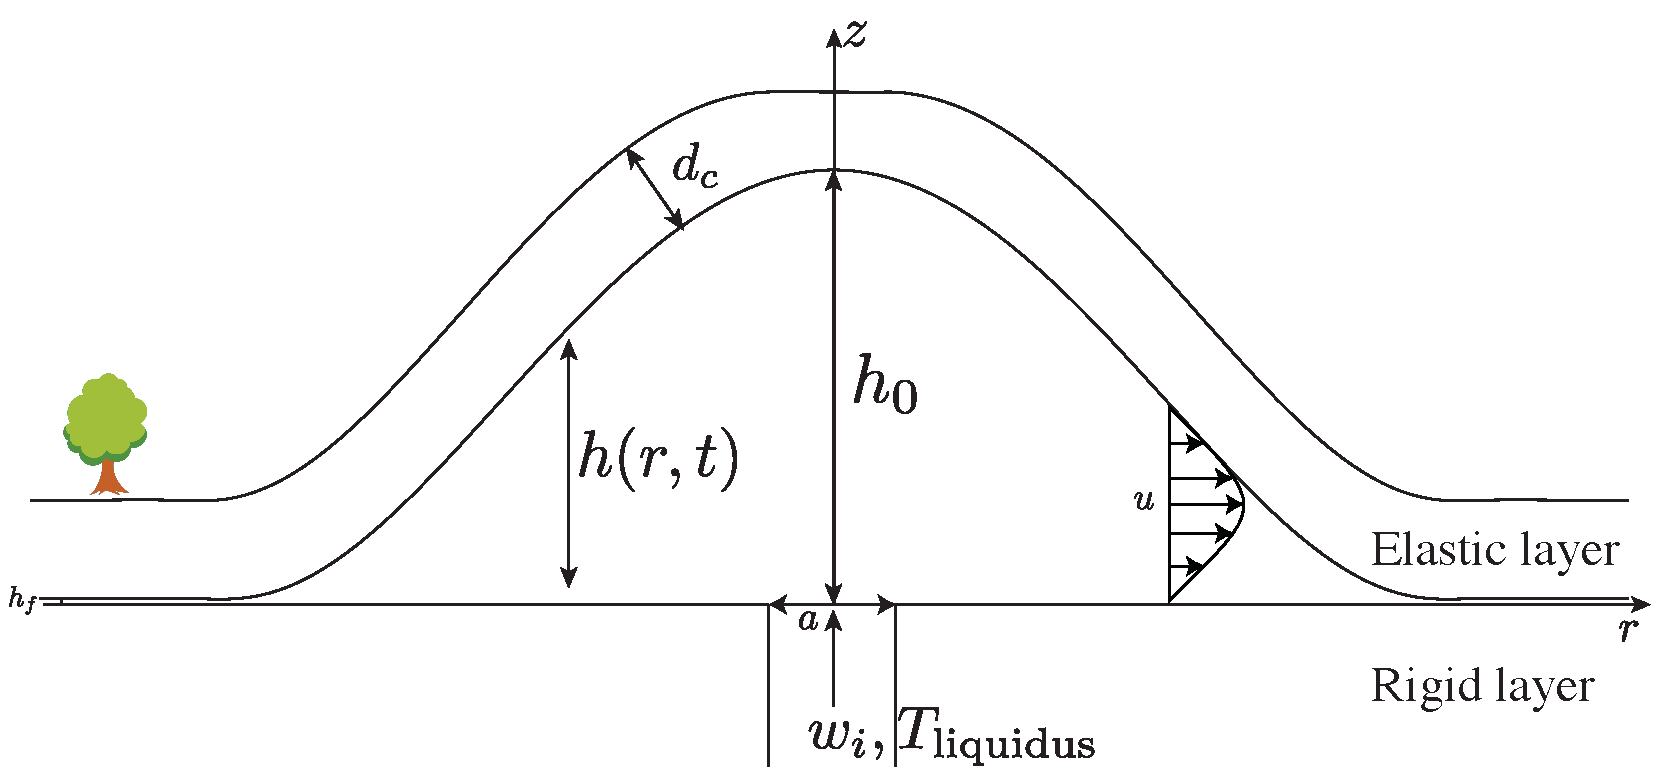
\includegraphics[scale=0.40]{C2_Sketch.pdf}
    \caption{Model geometry and parameters.}
    \label{C2-Sketch}
  \end{center}
\end{figure}

\subsection{Governing equation}
\label{C2-sec:Governing equation}

\textbf{Driving pressure}\\

The  intrusion develops  over a  length scale  $\Lambda$ that  is much
larger than its  thickness $H$ ($\epsilon = H/ \Lambda<<  1$).  In the
laminar  regime  and  in  axisymmetrical  coordinates  ($r$,$z$),  the
Navier-stokes equations within the lubrication assumption are
\begin{eqnarray}
  -\frac{\partial P}{\partial r}  +  \frac{\partial}{\partial z}\left(\eta \frac{\partial u}{\partial z}\right) &=&0\label{C2_V1} \\
  -\frac{\partial P}{\partial z}  - \rho_{m}g&  =&0\label{C2-Npressure}
\end{eqnarray}
where  $u(r,z,t)$  is  the  radial   velocity,  $g$  is  the  standard
acceleration due to gravity and  $P(r,z,t)$ is the pressure within the
fluid.   Integration  of  (\ref{C2-Npressure}) thus  gives  the  total
pressure  $P(r,z,t)$ within  the flow.   When the  vertical deflection
deflection $h(r,t)$  of the upper  elastic layer is small  compared to
its thickness  $d_c$, i.e $h<<d_c$,  we can neglect stretching  of the
upper layer and only consider  bending stresses.  Therefore, the total
pressure $P(r,z,t)$ at a level $z$ in the intrusion is the sum of four
contributions: the  weight of the  magma and  of the upper  layer, the
bending pressure $P_b$ and the atmospheric pressure $P_0$
\begin{equation}
  P = \rho_m g (h-z)+\rho_rgd_c+P_b+P_0
  \label{C2-pression}
\end{equation}
where $h(r,t)$ is the intrusion  thickness and $\rho_r$ the density of
the surrounding rocks. The bending pressure  is given by the force per
unit area  that is necessary  for a  vertical displacement $h$  of the
thin elastic plate \citep{Turcotte:1982ca}
\begin{equation}
  P_d = D\nabla^4h
\end{equation}
where $D$  is the flexural  rigidity of  the thin elastic  layer, that
depends on the Young's modulus $E$, Poisson's ratio $\nu^*$ and on the
elastic           layer          thickness           $d_c$          as
$D = Ed_c^3/\left(12(1-\nu^*)\right)$.

\vspace{.5cm} \textbf{Velocity field} \vspace{.5cm}

At the contact with the elastic sheet $z=h(r,t)$, the no-slip boundary
condition is present  and so, the tangential velocity is  zero and the
normal velocity  is the change  in height ($\partial h/  \partial t$).
With $\vec{n}$ the normal to the surface and $\vec{t}$ the tangent, we
have
\begin{eqnarray}
  \vec{n} \cdot (u,w) &=& \frac{\partial h }{\partial t}\\
  \vec{t} \cdot (u,w) &=& 0 \label{tangeant}.
\end{eqnarray}
The  tangent  vector is  $\vec{t}  =  (1,  \partial h/  \partial  r)$.
However, within the lubrication  assumption, the vertical component of
the  tangent  vector scales  as  $\epsilon$  and thus,  is  negligible
compared to  the radial  component. Therefore, the  boundary condition
($\ref{tangeant}$) reduces  to $u(r,z=h,t)  =0$.  At  the base  of the
flow, the same boundary condition hold and $u(r,z=0,t) =0$.

Equation (\ref{C2_V1}) is integrated twice  as a function of $z$ using
these boundary conditions and the horizontal velocity is
\begin{equation}
  u(r,z,t) =\frac{1}{2\eta} \frac{\partial P}{\partial r} \left(z^2-hz\right)
  \label{C2-vel}
\end{equation}

\vspace{.5cm} \textbf{Injection rate} \vspace{.5cm}

The effective overpressure $\Delta P^*$ driving the flow in the feeder
conduit decreases as the intrusion thickens and is given by
\begin{equation}
  \Delta P^* = \Delta P -\rho_m g h_0 \label{C2-Q0}
\end{equation}
where $h_0(t)$ is the maximum  intrusion thickness at the center $r=0$
and $\Delta P$ is the initial  driving pressure or the overpressure at
the base of the dyke ($z = -Z_c$).

In (\ref{C2-Q0}), the bending pressure  at then center, which scale as
D$h_0(t)/R(t)^4$  where  $R(t)$  is   the  blister  radius,  has  been
neglected.  Although  it tends  to infinity at  the initiation  of the
flow, it rapidly  vanishes as the blister spreads  and the hydrostatic
pressure $\rho_m g h_0$ becomes  the main contribution to the pressure
at the  center.  In addition, the  model assumes a large  aspect ratio
for the blister and does not consider the initiation of the flow.

Finally,  assuming a  Poiseuille flow  within the  cylindrical feeding
conduit, the vertical injection velocity $w_i(r,t)$ and injection rate
$Q(t)$ are given by
\begin{equation}
  w_i=
  \begin{cases}
    \frac{ \Delta P^*}{4 \mu Z_{c}} (\frac{a^{2}}{4}-r^{2})& r \le \frac{a}{2}\\
    0 & r > \frac{a}{2}
  \end{cases}
  \label{C2-eq12}
\end{equation}
\begin{equation}
  Q = Q_0(1-\frac{\rho_m g h_0}{\Delta P})
  \label{C2-eq11}
\end{equation}
where
$Q_0=\left(\pi \Delta P^* a^{4}\right)/\left(128 \eta Z_c\right)$.

\vspace{.5cm} \textbf{Mass conservation} \vspace{.5cm}

The fluid  is assumed  incompressible and a  global statement  of mass
conservation gives
\begin{eqnarray}
  \frac{\partial         h}{\partial        t} +\frac{1}{r}
  \frac{\partial}{\partial
  r} \left( r\int_0^hudz\right) = w_i
  \label{C2-Mass}
\end{eqnarray}
and using (\ref{C2-vel}), we find  that the equation for the evolution
of the thickness in time and space reads
\begin{equation}
  \frac{\partial h}{\partial t} =\frac{\rho_mg}{12 \eta r}
  \frac{\partial}{\partial r}  \left( rh^3  \frac{\partial h}{\partial
      r}\right)+\frac{D}{12\eta r} \left( rh^3 \frac{\partial}{\partial r}\nabla^4h\right)+
  w_i .\label{C2-Heq}
\end{equation}
It is  composed of three different  terms on the right  hand side. The
first term represents gravitational  spreading, i.e.  spreading of the
blister under its own weight. The second term represents the squeezing
of the  flow by the upper  elastic layer.  Both term  are negative and
induces spreading.   The last term  represents fluid injection  and is
positive.

\subsection{Dimensionless equations}
\label{C2-sec:dimens-equat}

Equations  (\ref{C2-eq12}) and  (\ref{C2-Heq}) are  nondimensionalized
using a  horizontal scale $\Lambda$, a  vertical scale $H$ and  a time
scale $\tau$ given by
\begin{eqnarray}
  \Lambda &=& \left(\frac{D}{\rho_m g}\right)^{1/4}\label{L1}\\
  H&=&\left       (\frac{12\eta      Q_{0}}{\rho_{m}g       \pi}\right      )
       ^{\frac{1}{4}} \label{H1}\\
  \tau&=&\frac{\pi \Lambda^{2} H}{Q_{0}}\label{T1}
\end{eqnarray}

where scales  are chosen  such that $Q_0  = \pi\Lambda^2  H/\tau$. The
length scale $\Lamba$ represents the  flexural wavelength of the upper
elastic layer,  i.e. the  length scale at  which bending  stresses and
gravity  contributes equally  to flow.   The height  scale $H$  is the
thickness of  a typical gravity current  and the time scale  $\tau$ is
the  characteristic time  to  fill  up a  cylindrical  flow of  radius
$\Lambda$ and thickness  $H$ at constant rate $Q_0$.   In addition, we
can       define        a       horizontal        velocity       scale
$U=\Lambda/\tau=\left(\rho_m           g           H^3\right)/\left(12
  \eta_h\Lambda\right)$.

The dimensionless equation is
\begin{eqnarray}
  \frac{\partial h}{\partial t}& =&\frac{1}{ r}
                                    \frac{\partial}{\partial r}  \left( rh^3  \frac{\partial h}{\partial
                                    r}\right)+\frac{1}{ r} \left( rh^3
                                    \frac{\partial}{\partial
                                    r}\nabla^4h\right)\nonumber\\
                               &+&
                                   \frac{32}{\gamma^{2}}\left(\frac{1}{4}-\frac{r^{2}}{\gamma^{2}}\right)\left(1-\frac{h_0}{\sigma}\right)
                                   \label{C2-mainEq}
\end{eqnarray}
where the last term is replaced by zero for $r>\gamma/2$. $\gamma$ and
$\sigma$ are  two dimensionless numbers  that control the  dynamics of
the flow
\begin{eqnarray}
  \gamma &=& \frac{a}{\Lambda}\\
  \sigma &=& \frac{\Delta P}{\rho_m g h}.
\end{eqnarray}
$\gamma$  is the  dimensionless radius  of  the conduit,  it does  not
significantly influence the flow and is set to $0.02$ in the following
\citep{Michaut:2009jx,Michaut:2011kg}.   $\sigma$  is  the  normalized
pressure  head,  i.e.,  the  ratio between  the  initial  overpressure
driving the flow and the weight of the magma at the center.
	 
\subsection{Need for regularization}
\label{C2-sec:need-regularization}

One  of   the  main   mathematical  difficulty  in   solving  equation
(\ref{C2-mainEq}) arises at the  contact line.  Indeed, the assumption
that the  thickness of  the fluid  tends to zero  at the  contact line
leads  to  divergent  viscous  stresses, and  hence,  the  theoretical
immobility                of                the                blister
\citep{Flitton:1999iv,Lister:2013ia,Anonymous:QWXp_4JV}. This problem,
known  a  the  contact-line  paradox,  is  a  well  know  problem  for
surface-tension driven flow  such as the spreading of  a water droplet
\citep{Bertozzi:1998wz,Snoeijer:2013cm}.

The formal proof  have been derived by  \citet{Flitton:1999iv} and can
be derived  as follow. Suppose  that (\ref{C2-mainEq}) has  a solution
and the solution has the  form $h \sim A(t)(R(t)-r)^{\alpha}$ near the
contact line.  As $r \rightarrow R(r)$, the bending term dominates the
gravitational term and (\ref{C2-mainEq}) reduces to
\begin{eqnarray}
  \frac{\partial       h}{\partial       t}&      =&\frac{1}{       r}
                                                     \frac{\partial}{\partial r}\left( rh^3 \frac{\partial}{\partial r}\nabla^4h\right).
                                                     \label{C2-mainEq2}
\end{eqnarray}
Injecting the  solution into  (\ref{C2-mainEq2}) and keeping  only the
leading powers of $R-r$ gives
\begin{eqnarray}
  \frac{\partial    R}{\partial    t}    A\alpha\left(R-r\right)^{\alpha-1}+
  \frac{\partial           A}{\partial           t}\left(R-r)^{\alpha}
  &=&A^4\alpha(\alpha-1)(\alpha-2)\nonumber\\
  &&(\alpha-3)(\alpha-4)(\alpha-5)(R-r)^{4\alpha-6}\nonumber
\end{eqnarray}
The second  term on  the left is  small compared to  the first  as the
blister  grows  mainly by  spreading  at  the  tip and  therefore,  by
equating  the exponent  of $R-r$,  we obtain  $\alpha =  5/3$, and  by
equating the coefficients, we deduce
\begin{equation}
  \frac{\partial R}{\partial r} =-\frac{280}{243} A^3.
\end{equation}
It shows that (\ref{C2-mainEq}) can  only have retreating contact line
($dR/dt<0$)   but  not   with  advancing   contact  line   ($dR/dt>0$)
\citep{Lister:2013ia,Flitton:1999iv}.

To  mitigate this  problem,  one  common approach  is  to  add a  thin
pre-wetting film, with thickness $h_f$ such that $h\rightarrow h_f$ as
$r\rightarrow  \infty$.   While  the  solution will  depend  upon  the
pre-wetted  film thickness  $h_f$ and  will not  show any  convergence
properties when $h_f\rightarrow 0$, we will see that the dependence in
$h_f$ is  weak and the  difference between different values  for $h_f$
will  be  relatively  small  \citep{Lister:2013ia,Anonymous:QWXp_4JV}.
Unless otherwise specified, we will consider $h_f = 5\cdot 10^{-3}$ in
the manuscript.



\section{Regime of propagations}
\label{C2-sec:regime-propagations}

For  a  small  pre-wetting   film  thickness,  i.e.   $h_f/H<<1$,  the
numerical  resolution of  the  equation  (\ref{EqFinal1}) shows  three
spreading regimes:  a bending  regime where  gravity is  negligible, a
viscous  gravity current  regime  where bending  is  negligible and  a
regime               of              lateral               propagation
\citep{Michaut:2011kg,Bunger:2011cb,Lister:2013ia}.

\begin{figure}[h!]
  \begin{center}
    \graphicspath{ {/Users/thorey/Documents/These/Manuscript/Figure/Chapter2/} }
    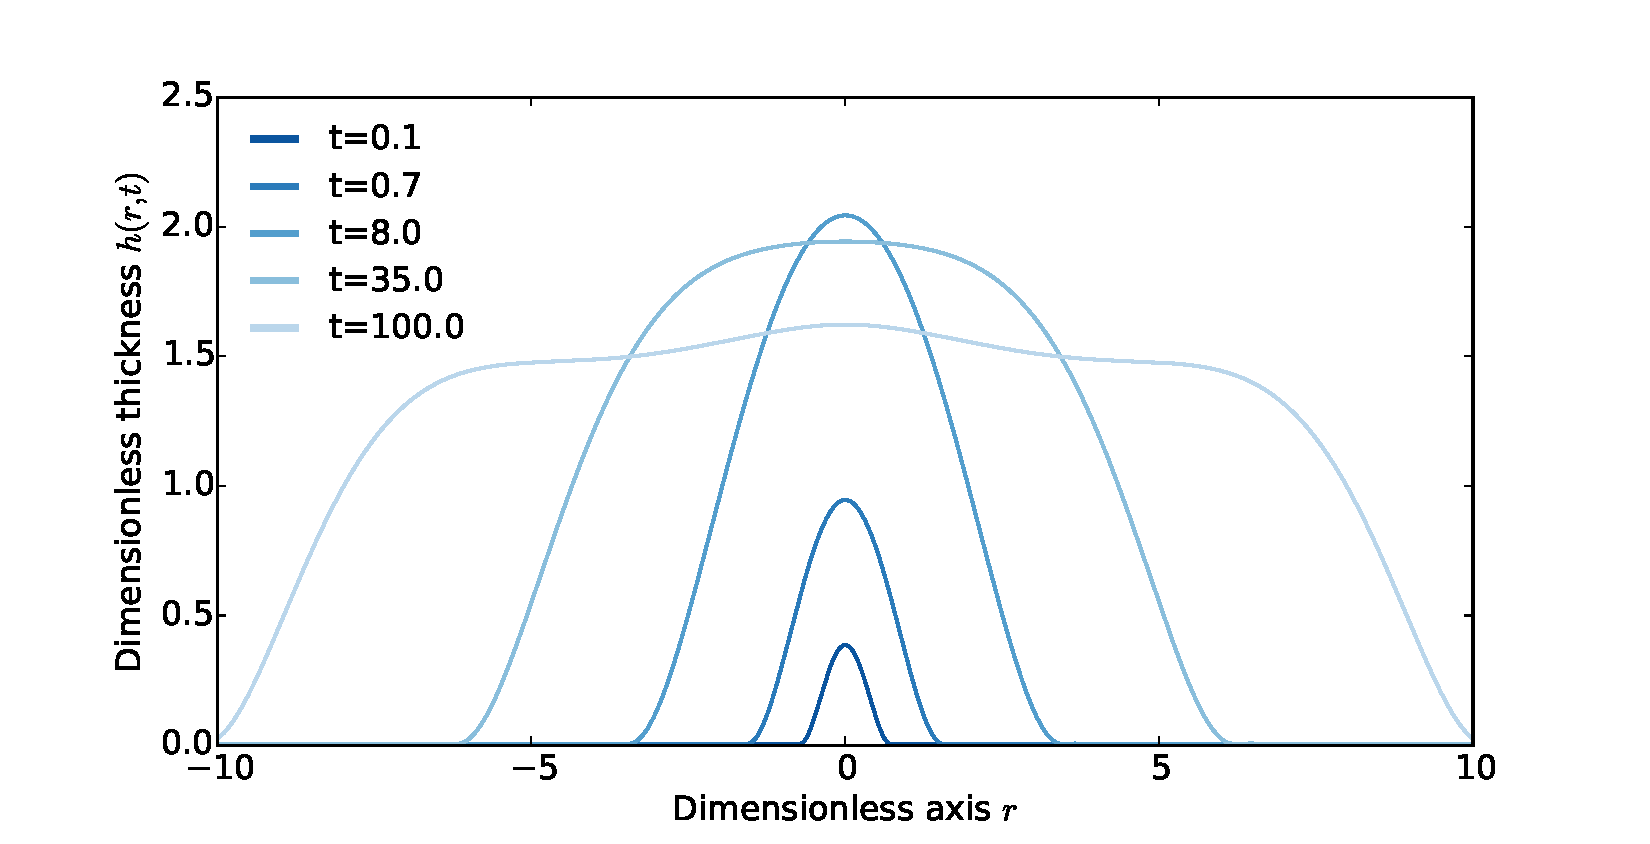
\includegraphics[scale=0.5]{C2_ELAS_GRAV_Profil.eps}
    \caption{Shape of the flow, i.e.  thickness $h(r,t)$ as a function
      of the radial axis $r$ at  five different times indicated on the
      plot. Variables are  dimensionless and one needs  to multiply by
      the characteristic  scales (thickness,  length or time  given by
      (\ref{H1}),  (\ref{L1})  or  (\ref{T1})) to  obtain  dimensional
      values.  For $t<10$,  the  intrusion is  in  the bending  regime
      whereas  for $t>10$  the  intrusion is  in  the gravity  current
      regime.}
    \label{C2_ELAS_GRAV_Profil}
  \end{center}
\end{figure}

\subsection{Bending regime}
\label{C2-sec:bending-regime}

At  early times,  when  $R<<\Lambda$, gravity  is  negligible and  the
dynamics of  the spreading  is governed  by the  bending of  the upper
layer.   In addition,  if $h_0<<\sigma$,  the overpressure  $\Delta P$
driving the flow is much larger than  the weight of the blister at the
center and the injection rate can be considered constant.

In that case, the spreading is  very slow and the interior has uniform
pressure $P =\nabla^4h$.  The flow is bell-shaped and its thickness is
given by
\begin{equation}
  h(r,t) = h_0(t)\left(1-\frac{r^2}{R^2(t)}\right)^2
  \label{IntrusionShape}
\end{equation}
with  $h_0(t)$   the  thickness  of   the  intrusion  at   the  center
\citep{Michaut:2011kg,Lister:2013ia}.       In       this      regime,
\citet{Lister:2013ia} have  shown that the spreading  is controlled by
the propagation  of a peeling by  bending wave at the  intrusion front
with dimensionless velocity $c$
\begin{equation}
  c=    \frac{\partial             R}{\partial            t}             =h_f^{1/2}
  \left(\frac{\kappa}{1.35}\right)^{5/2}
  \label{WaveVelocity}
\end{equation}
where  $\kappa  =  \partial^2  h/\partial r^2$  is  the  dimensionless
curvature  of  the  interior  solution.   Using  the  propagation  law
(\ref{WaveVelocity})   and  the   form   of   the  interior   solution
(\ref{IntrusionShape}), they  find that the  radius and the  height of
the intrusion are given by similarity solutions
\begin{eqnarray}
  R(t) &=& 2.2h_f^{1/22}t^{7/22}\label{ScalingR}\\
  h_0(t)&=&0.67 h_f^{-1/11}t^{8/22}\label{ScalingH}.
\end{eqnarray}
where the numerical pre-factor have been matched to our simulations.

\begin{figure}
  \begin{center}
    \graphicspath{ {/Users/thorey/Documents/These/Manuscript/Figure/Chapter2/} }
    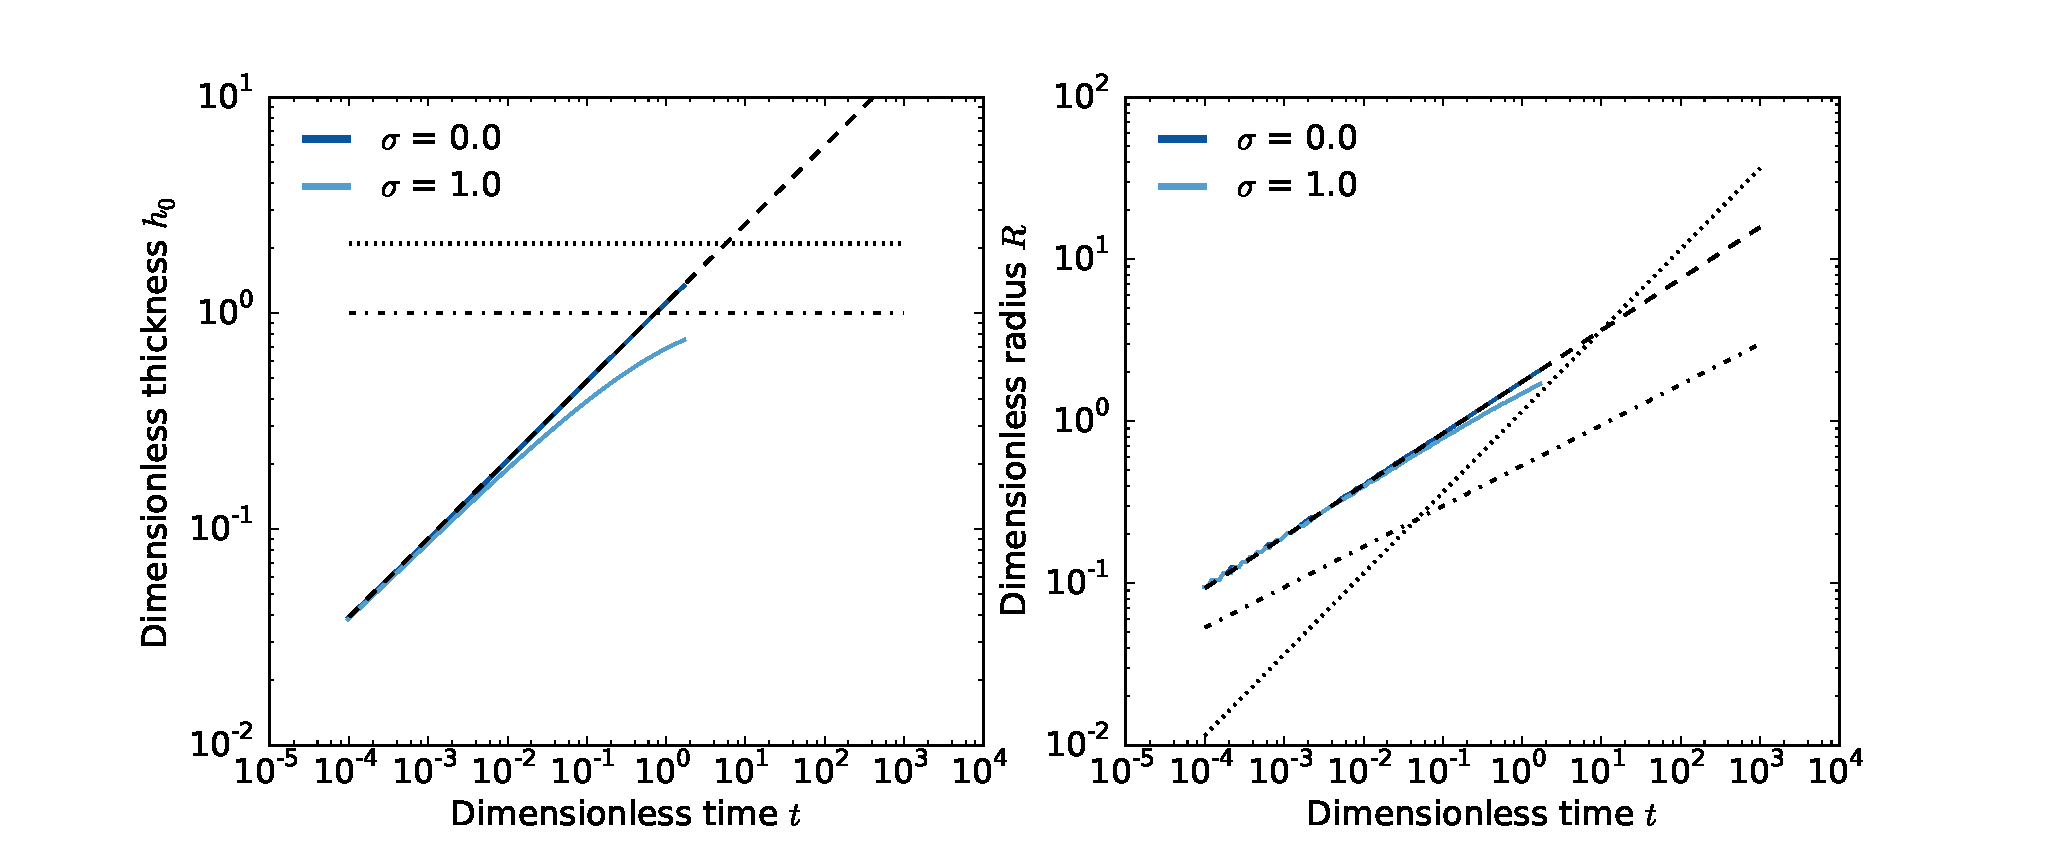
\includegraphics[scale=0.4]{C2_ELAS_GRAV_Sigma.eps}
    \caption{Left: Dimensionless thickness at  the center $h_0$ versus
      dimensionless  time  $t$   for  different  dimensionless  number
      $\sigma$  indicated on  the  plot.   Dashed-lines represent  the
      scaling  laws in  the different  regimes.  Right:  Dimensionless
      radius  $R$   versus  dimensionless   time  $t$  for   the  same
      dimensionless  number  $\sigma$.    Dashed-lines  represent  the
      scaling laws in the different regimes.}
    \label{C2_ELAS_GRAV_Sigma}
  \end{center}
\end{figure}

\subsection{Gravity current regime}
\label{C2-sec:grav-curr-regime}

In  contrast, when  the radius  R becomes  much larger  than $\Lambda$
($R>>\Lambda$), the weight of the  intrusion becomes dominant over the
bending  terms.  The  pressure is  given by  the hydrostatic  pressure
$P = h$  and the intrusion enters a classical  viscous gravity current
regime where bending terms only affect the solution near the intrusion
edge   \citep{Huppert:1982a,Michaut:2011kg,Lister:2013ia}.   In   this
second regime, the radius evolves as $t^{1/2}$ and the thickness tends
to a constant
\begin{eqnarray}
  R(t) &=& 0.715 t^{1/2}\label{Scaling-R-Gravi}\\
  h_0 &=& 1.86\label{Scaling-H-Gravi}
\end{eqnarray} 

\subsection{Lateral propagation}
\label{sec:lateral-propagation}

Once $h_0\rightarrow \sigma$,  the flow is thick  enough to compensate
for  the initial  overpressure. The  thickness at  the center  remains
constant and  the flow enters  a regime of lateral  propagation, where
only its radius $R(t)$ is  to increase \citep{Michaut:2011kg}. In this
regime, except at the center when it redistributes the pressure over a
length scale $\Lambda$, the bending term is negligible compared to the
gravitational  term. \citet{Michaut:2011kg}  has  shown  that in  this
regime, the thickness is constant and the radius evolves as $t^{1/4}$
\begin{eqnarray}
  R(t) &=& \left(\frac{\sigma^3 t}{4\pi}\right)^{1/4}\label{Scaling-R-Propa}\\
  h_0 &=& \sigma\label{Scaling-H-Propa}
\end{eqnarray} 

\section{Application to laccoliths}
\label{C2-sec:appl-earth-moon}

In the following, we apply the isoviscous-gravity current.
\begin{figure}
  \begin{center}
    \graphicspath{ {/Users/thorey/Documents/These/Manuscript/Figure/Chapter2/} }
    \includegraphics[scale=0.35]{C2_Geological_Data.eps}
    \caption{}
    \label{C2_Geological_Data}
  \end{center}
\end{figure}


\section{Discussion}
\label{C2-sec:discussion}


\begin{table}
  \caption{Range of values for the model parameters}
  \centering
  \begin{tabular}{c|c|c|c}
    \hline
    Parameters& Symbol & Range of values &Unit\\
    \hline
              &&\\
    Depth of intrusion & $d_c$ & $0.1-5$ &km \\
    Young's Modulus & $E$ & $10-100$ &GPa \\
    Poisson's ratio & $\nu^*$ & $0.25$ &\\
    Gravity & $g$ & $9.81$ &m s$^{-2}$ \\
    Magma density & $\rho_{m}$ & $2800-3200$ &kg m$^{-3}$ \\
    Magma viscosity & $\eta $ & $1-10^{4}$ &Pa s \\
    Feeder dyke width & $a$ & $1-100$ &m \\
    Depth of the melt source & $Z_{c}$ & $ 5-500$& km \\ 
    Initial overpressure & $\Delta P$ & $5-50$ &MPa \\
    Injection rate & $Q_{0}$ &$10p{-3}-0.1$ &m$^{3}$ s$^{-1}$ \\
    Crust density & $\rho_{r}$ & $2500$ &kg m$^{-3}$ \\
              &&\\
    \hline
    Characteristic scales & Symbol & Range of values & Unit\\
    \hline
              &&\\
    Height scale & $H$& $0.1-10$ &m \\
    Length scale & $\Lambda$ & $1-12$& km \\
    Time scale & $\tau$ & $10^{-1}-10$ &years \\
    \label{tab2}
  \end{tabular} 
\end{table}
\begin{table}
  \caption{Dimensionless numbers}
  \centering
  \begin{tabular}{c|c|c|c}
    &&Complex craters&Simple craters \\
    \hline
    Symbol& Description & Range of values & Range of values \\
    \hline
    &&\\
    $\gamma$&Normalized source width& $10^{-4}-10^{-2}$ &$10^{-4}-10^{-2}$ \\
    $\zeta$& Normalized wall zone width  & $0.05-0.13$&$0.25$\\
    $\Psi$&Thickening term & $0.3-8$&$0.2-4$\\
    $\Xi$& Hydrostatic term & $20-400$&$20-200$\\
    $\Theta$ &Elastic term & $10^{-7}-0.1$&$10^{-3}-10$\\
    $\Omega$ & Density ratio & $1.2$ &$1.2$\\
    $\Phi$ & Upper layer aspect ratio & $4500$ &$1200 $\\
    $\sigma$&Normalized pressure head& $0.6-100$ & $0.6-100$ 
                                                   \label{tab3}
  \end{tabular} 
  % \tablenotetext{a}{Footnote text here.}
\end{table}

\bibliographystyle{agufull08}
\bibliography{/Users/thorey/Dropbox/Library}



%%% Local Variables:
%%% mode: latex
%%% TeX-master: "../main"
%%% End:
